\documentclass[aspectratio=1610, 11pt]{beamer}

% ── Theme & Colors ──────────────────────────────────────────────
\usetheme{Madrid}
\usecolortheme{whale}
\definecolor{edcblue}{RGB}{0,90,156}
\definecolor{edcgreen}{RGB}{46,139,87}
\definecolor{edcorange}{RGB}{210,105,30}
\definecolor{edcred}{RGB}{178,34,34}
\definecolor{lightgray}{RGB}{240,240,240}
\setbeamercolor{structure}{fg=edcblue}
\setbeamercolor{frametitle}{bg=edcblue!90!black, fg=white}
\setbeamercolor{title}{fg=white, bg=edcblue}
\setbeamercolor{block title}{bg=edcblue!80, fg=white}
\setbeamercolor{block body}{bg=edcblue!5}
\setbeamercolor{block title alerted}{bg=edcorange!80, fg=white}
\setbeamercolor{block body alerted}{bg=edcorange!5}
\setbeamercolor{block title example}{bg=edcgreen!70, fg=white}
\setbeamercolor{block body example}{bg=edcgreen!5}

\setbeamertemplate{navigation symbols}{}
\setbeamertemplate{footline}{%
  \leavevmode\hbox{%
    \begin{beamercolorbox}[wd=.33\paperwidth,ht=2.5ex,dp=1ex,center]{author in head/foot}%
      \usebeamerfont{author in head/foot}Yinuo Sheng
    \end{beamercolorbox}%
    \begin{beamercolorbox}[wd=.34\paperwidth,ht=2.5ex,dp=1ex,center]{title in head/foot}%
      \usebeamerfont{title in head/foot}FedGen
    \end{beamercolorbox}%
    \begin{beamercolorbox}[wd=.33\paperwidth,ht=2.5ex,dp=1ex,right]{date in head/foot}%
      \usebeamerfont{date in head/foot}\insertframenumber{}/\inserttotalframenumber\hspace*{2em}
    \end{beamercolorbox}}%
}

% ── Packages ────────────────────────────────────────────────────
\usepackage{tikz}
\usetikzlibrary{arrows.meta, positioning, shapes.geometric, fit, calc, decorations.pathreplacing}
\usepackage{booktabs}
\usepackage{fontspec}
\usepackage{graphicx}
\usepackage{listings}
\usepackage{xcolor}
\usepackage{adjustbox}

\lstset{
  basicstyle=\ttfamily\tiny,
  breaklines=true,
  frame=single,
  backgroundcolor=\color{lightgray},
  columns=fullflexible,
}

% ── Meta ────────────────────────────────────────────────────────
\title[FedGen]{FedGen: A Sovereign Dataspace for\\Decentralized AI Training Corpora}
\subtitle{CSC4240/CSC6203 Data Spaces --- Final Project}
\author{Yinuo Sheng \quad 122090461}
\date{Spring 2026}
\institute{}

% ════════════════════════════════════════════════════════════════
\begin{document}

% ── Slide 1: Title ──────────────────────────────────────────────
\begin{frame}[plain]
\titlepage
\begin{center}
\small\textit{How can organizations share training data for AI\\while retaining full control over access and usage?}
\end{center}
\end{frame}

% ── Slide 2: Project Evolution ──────────────────────────────────
\begin{frame}{Project Evolution}
\begin{columns}[T]
\begin{column}{0.48\textwidth}
\begin{block}{Original Proposal}
\begin{itemize}
  \item 4-node EDC dataspace
  \item Sample legal \& news datasets
  \item Contract negotiation demo
  \item Federated catalog discovery
\end{itemize}
\end{block}
\end{column}
\begin{column}{0.48\textwidth}
\begin{alertblock}{Semester Extensions}
\begin{itemize}
  \item[\textcolor{edcorange}{\textbf{+}}] \textbf{Third-party database} access\\(Wikidata SPARQL integration)
  \item[\textcolor{edcorange}{\textbf{+}}] \textbf{Federated learning} demo\\(FedAvg from scratch in NumPy)
  \item[\textcolor{edcorange}{\textbf{+}}] Live API proxying\\(OpenAlex, Hacker News)
\end{itemize}
\end{alertblock}
\end{column}
\end{columns}
\vspace{0.5em}
\begin{center}

\begin{tikzpicture}
  \draw[-{Stealth[length=3mm]}, very thick, edcblue]
    (0,0) node[left, font=\small\bfseries]{Proposal} -- (5,0) node[right, font=\small\bfseries]{Final System};
  \foreach \x/\lab in {1.2/Live APIs, 2.7/Wikidata, 4.2/FedAvg}{
    \fill[edcorange] (\x,0) circle(3pt);
    \node[above, font=\tiny] at (\x,0.15) {\lab};
  }
\end{tikzpicture}
\end{center}
\end{frame}

% ── Slide 3: Architecture Overview ──────────────────────────────
\begin{frame}{Architecture Overview}
\begin{center}
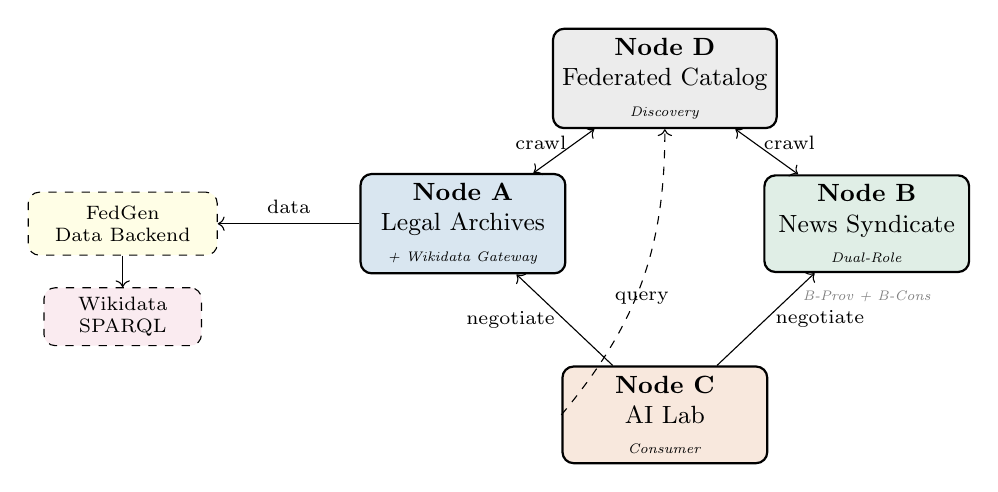
\begin{tikzpicture}[
  node distance=1.2cm and 2.2cm,
  box/.style={draw, rounded corners, minimum width=2.6cm, minimum height=1.1cm, font=\small, align=center, thick},
  every edge/.style={draw, -{Stealth[length=2.5mm]}, thick},
]
  % Nodes
  \node[box, fill=edcblue!15] (A) {\textbf{Node A}\\Legal Archives\\{\tiny\textit{+ Wikidata Gateway}}};
  \node[box, fill=edcgreen!15, right=2.5cm of A] (B) {\textbf{Node B}\\News Syndicate\\{\tiny\textit{Dual-Role}}};
  \node[box, fill=edcorange!15, below=1.8cm of $(A)!0.5!(B)$] (C) {\textbf{Node C}\\AI Lab\\{\tiny\textit{Consumer}}};
  \node[box, fill=gray!15, above=1.2cm of $(A)!0.5!(B)$] (D) {\textbf{Node D}\\Federated Catalog\\{\tiny\textit{Discovery}}};

  % Backend
  \node[draw, dashed, rounded corners, fill=yellow!10, minimum width=2.4cm, minimum height=0.8cm, font=\scriptsize, align=center, left=1.8cm of A] (BE) {FedGen\\Data Backend};
  \node[draw, dashed, rounded corners, fill=purple!8, minimum width=2.0cm, minimum height=0.7cm, font=\scriptsize, align=center, below=0.4cm of BE] (WD) {Wikidata\\SPARQL};

  % Edges
  \draw[->] (C) -- node[left, font=\scriptsize]{negotiate} (A);
  \draw[->] (C) -- node[right, font=\scriptsize]{negotiate} (B);
  \draw[<->] (D) -- node[left, font=\scriptsize, pos=0.3]{crawl} (A);
  \draw[<->] (D) -- node[right, font=\scriptsize, pos=0.3]{crawl} (B);
  \draw[->, dashed] (C.west) to[bend right=20] node[below, font=\scriptsize]{query} (D.south);
  \draw[->] (A) -- node[above, font=\scriptsize]{data} (BE);
  \draw[->] (BE) -- (WD);

  % B dual-role annotation
  \node[font=\tiny\itshape, text=gray, below=0.1cm of B] {B-Prov + B-Cons};
\end{tikzpicture}
\end{center}
\vspace{-0.3em}
\small Infrastructure: Kubernetes (k3d) + Terraform + Eclipse MVD + custom Python backend
\end{frame}

% ── Slide 4a: Core Scenario — Lifecycle ─────────────────────────
\begin{frame}[fragile]{Data Sharing Lifecycle (Scenario 1: C \texorpdfstring{$\to$}{->} A)}
\vspace{-0.5em}
\begin{center}
\resizebox{0.92\textwidth}{!}{%
\begin{tikzpicture}[
  step/.style={draw, rounded corners, minimum width=1.6cm, minimum height=0.55cm, font=\scriptsize, align=center, thick},
  arr/.style={-{Stealth[length=2mm]}, thick},
]
  % Row 1: Provider setup
  \node[step, fill=edcblue!12] (s1) at (0,0) {Register Asset};
  \node[step, fill=edcblue!12] (s2) at (2.5,0) {Create Policy};
  \node[step, fill=edcblue!12] (s3) at (5.0,0) {Contract Def};
  \draw[arr] (s1) -- (s2);
  \draw[arr] (s2) -- (s3);
  \node[above=0.08cm of s2, font=\scriptsize\bfseries, edcblue] {Provider (Node A)};

  % Row 2: Consumer negotiation
  \node[step, fill=edcgreen!12] (s4) at (0,-1.3) {Query Catalog};
  \node[step, fill=edcorange!15] (s5) at (2.5,-1.3) {Negotiation};
  \node[step, fill=edcorange!15] (s6) at (5.0,-1.3) {FINALIZED};
  \draw[arr] (s3) -- (s6);
  \draw[arr] (s4) -- (s5);
  \draw[arr] (s5) -- (s6);
  \node[above=0.08cm of s5, font=\scriptsize\bfseries, edcgreen] {Consumer (Node C)};

  % Row 3: Transfer
  \node[step, fill=edcred!12] (s7) at (0,-2.6) {HTTP-PULL};
  \node[step, fill=edcred!12] (s8) at (2.5,-2.6) {EDR Token};
  \node[step, fill=edcred!15] (s9) at (5.0,-2.6) {\textbf{Pull Data}};
  \draw[arr] (s6) -- (s9);
  \draw[arr] (s7) -- (s8);
  \draw[arr] (s8) -- (s9);
  \node[above=0.08cm of s8, font=\scriptsize\bfseries, edcred] {Transfer};

  % DCP callout to the right
  \node[draw, dashed, rounded corners, fill=gray!8, font=\scriptsize, align=left,
        text width=4.2cm] (dcp) at (8.8,-0.65) {
    \textbf{DCP Auth Flow:}\\
    1. Provider sends PresentationQuery\\
    \quad to Consumer Identity Hub\\
    2. IH returns VP with\\
    \quad MembershipCredential\\
    3. Provider verifies \& evaluates\\
    \quad ODRL policy
  };
  \draw[->, dashed, gray] (s5.east) -- (dcp.west);
\end{tikzpicture}%
}
\end{center}
\end{frame}

% ── Slide 4b: Other Scenarios ───────────────────────────────────
\begin{frame}{Other Core Scenarios}
\begin{columns}[T]
\begin{column}{0.32\textwidth}
\begin{block}{Scenario 2: C $\to$ B}
\small News data transfer with \textbf{DataAccess.level} obligation policy.\\[0.3em]
{\scriptsize Separate access + contract policies demonstrate ODRL flexibility.}
\end{block}
\end{column}
\begin{column}{0.32\textwidth}
\begin{exampleblock}{Scenario 3: Fed.\ Catalog}
\small Node D crawls A \& B catalogs $\to$ unified discovery for Node C.\\[0.3em]
{\scriptsize Consumer queries one endpoint to find all assets.}
\end{exampleblock}
\end{column}
\begin{column}{0.32\textwidth}
\begin{alertblock}{Scenario 4: Dual-Role}
\small B-Cons acquires legal data from A $\to$ same entity is both provider and consumer.\\[0.3em]
{\scriptsize Two connector instances, one logical domain.}
\end{alertblock}
\end{column}
\end{columns}
\vspace{0.8em}
\begin{center}
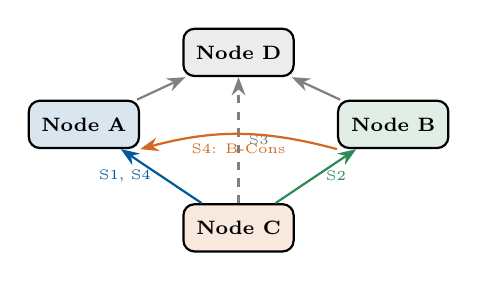
\begin{tikzpicture}[
  n/.style={draw, rounded corners, minimum width=1.4cm, minimum height=0.6cm, font=\scriptsize\bfseries, thick},
]
  \node[n, fill=edcblue!15] (a) {Node A};
  \node[n, fill=edcgreen!15, right=2.5cm of a] (b) {Node B};
  \node[n, fill=edcorange!15, below=1cm of $(a)!0.5!(b)$] (c) {Node C};
  \node[n, fill=gray!15, above=0.6cm of $(a)!0.5!(b)$] (d) {Node D};

  \draw[-{Stealth}, thick, edcblue] (c) -- node[left, font=\tiny]{S1, S4} (a);
  \draw[-{Stealth}, thick, edcgreen] (c) -- node[right, font=\tiny]{S2} (b);
  \draw[-{Stealth}, thick, gray, dashed] (c.north) -- node[right, font=\tiny]{S3} (d.south);
  \draw[-{Stealth}, thick, edcorange] (b.south west) to[bend right=15] node[below, font=\tiny]{S4: B-Cons} (a.south east);
  \draw[{Stealth}-, thick, gray] (d) -- (a);
  \draw[{Stealth}-, thick, gray] (d) -- (b);
\end{tikzpicture}
\end{center}
\end{frame}

% ── Slide 5: Third-Party Database ───────────────────────────────
\begin{frame}{Extension 1: Third-Party Database Integration}
\vspace{-0.2em}
\begin{center}
\resizebox{0.95\textwidth}{!}{%
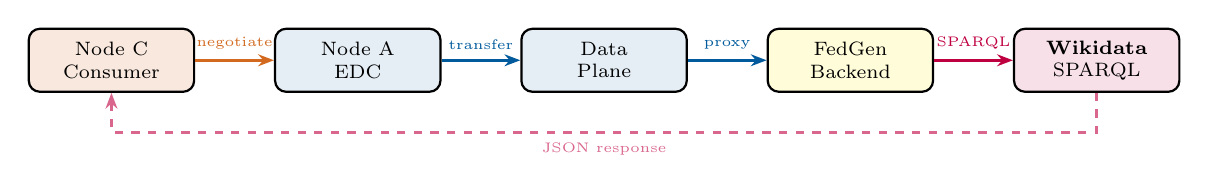
\begin{tikzpicture}[
  box/.style={draw, rounded corners, minimum width=2.1cm, minimum height=0.8cm, font=\scriptsize, align=center, thick},
  arr/.style={-{Stealth[length=2mm]}, very thick},
]
  \node[box, fill=edcorange!15] (consumer) {Node C\\Consumer};
  \node[box, fill=edcblue!10, right=1.0cm of consumer] (edc) {Node A\\EDC};
  \node[box, fill=edcblue!10, right=1.0cm of edc] (dp) {Data\\Plane};
  \node[box, fill=yellow!15, right=1.0cm of dp] (be) {FedGen\\Backend};
  \node[box, fill=purple!12, right=1.0cm of be] (wd) {\textbf{Wikidata}\\SPARQL};

  \draw[arr, edcorange] (consumer) -- node[above, font=\tiny]{negotiate} (edc);
  \draw[arr, edcblue] (edc) -- node[above, font=\tiny]{transfer} (dp);
  \draw[arr, edcblue] (dp) -- node[above, font=\tiny]{proxy} (be);
  \draw[arr, purple] (be) -- node[above, font=\tiny]{SPARQL} (wd);

  % Return path
  \draw[arr, purple!60, dashed] (wd.south) -- ++(0,-0.5) -| node[below, pos=0.25, font=\tiny]{JSON response} (consumer.south);
\end{tikzpicture}%
}

\vspace{0.2em}
{\scriptsize\itshape\color{gray} Same EDC flow as local data --- consumer \textbf{never} directly touches Wikidata}
\end{center}
\vspace{-0.2em}
\begin{columns}[T]
\begin{column}{0.48\textwidth}
\begin{block}{Backend Route: \texttt{/thirdparty/wikidata}}
\scriptsize
\begin{enumerate}\setlength\itemsep{0pt}
  \item Construct SPARQL query (AI/privacy concepts)
  \item Send to \texttt{query.wikidata.org}
  \item Transform JSON $\to$ FedGen format
  \item Cache result (5 min TTL)
\end{enumerate}
\end{block}
\end{column}
\begin{column}{0.48\textwidth}
\begin{exampleblock}{Verified Output (Real Data)}
\scriptsize
\begin{itemize}\setlength\itemsep{0pt}
  \item Q1172506 --- GDPR
  \item Q17233037 --- Cybersecurity
  \item Q23647168 --- Data protection
  \item Q11660 --- Artificial intelligence
  \item Q2539 --- Machine learning
\end{itemize}
\end{exampleblock}
\end{column}
\end{columns}
\end{frame}

% ── Slide 6: Federated Learning ─────────────────────────────────
\begin{frame}{Extension 2: Federated Learning (FedAvg)}
\vspace{-0.4em}
\begin{center}
\resizebox{0.92\textwidth}{!}{%
\begin{tikzpicture}[
  box/.style={draw, rounded corners, minimum width=2.4cm, minimum height=0.8cm, font=\small, align=center, thick},
  arr/.style={-{Stealth[length=2.5mm]}, thick},
]
  \node[box, fill=edcorange!15] (coord) at (0,0) {\textbf{Node C} Coordinator};
  \node[box, fill=edcblue!15] (na) at (-3.8,-2.4) {\textbf{Node A} Legal\\{\tiny 24 samples}};
  \node[box, fill=edcgreen!15] (nb) at (3.8,-2.4) {\textbf{Node B} News\\{\tiny 16 samples}};

  \draw[arr, edcorange] (coord.south west) -- node[left, font=\scriptsize, sloped, pos=0.45]{$W_{\text{global}}$} (na.north east);
  \draw[arr, edcorange] (coord.south east) -- node[right, font=\scriptsize, sloped, pos=0.45]{$W_{\text{global}}$} (nb.north west);
  \draw[arr, edcblue, dashed] (na.north) to[bend left=12] node[left, font=\scriptsize, pos=0.45]{$W_A, n_A$} (coord.west);
  \draw[arr, edcgreen, dashed] (nb.north) to[bend right=12] node[right, font=\scriptsize, pos=0.45]{$W_B, n_B$} (coord.east);

  \node[below=0.12cm of na, font=\tiny\itshape, text=edcblue] {Local SGD (3 epochs)};
  \node[below=0.12cm of nb, font=\tiny\itshape, text=edcgreen] {Local SGD (3 epochs)};
  \node[above=0.35cm of coord, font=\scriptsize] {$W_{\text{global}} \leftarrow \tfrac{n_A}{n_A+n_B} W_A + \tfrac{n_B}{n_A+n_B} W_B$};

  \node[draw, dashed, rounded corners, fill=edcred!5, font=\scriptsize, align=center,
        text width=3.4cm] (insight) at (8.2,-1.2) {
    \textbf{Key:} Raw text \textit{never}\\ leaves each node.\\ Only $W$ is exchanged.
  };
\end{tikzpicture}%
}
\end{center}
\vspace{-0.4em}
\begin{columns}[T]
\begin{column}{0.46\textwidth}
\begin{block}{Pipeline (all custom NumPy)}
\tiny
\begin{itemize}\setlength\itemsep{0pt}
  \item TF-IDF vectorizer (300 features)
  \item Logistic regression + mini-batch SGD
  \item Binary cross-entropy loss
  \item Non-IID partitioning (legal vs news)
\end{itemize}
\end{block}
\end{column}
\begin{column}{0.50\textwidth}
\begin{exampleblock}{Training Results (5 rounds, live data)}
\tiny
\begin{tabular}{cccc}
\toprule
\textbf{Round} & \textbf{Acc.} & \textbf{Loss A} & \textbf{Loss B} \\
\midrule
1 & 60\% & 0.574 & 0.551 \\
3 & 70\% & 0.468 & 0.579 \\
5 & \textbf{80\%} & 0.411 & 0.565 \\
\bottomrule
\end{tabular}
\end{exampleblock}
\end{column}
\end{columns}
\end{frame}

% ── Slide 7: Key Improvements ──────────────────────────────────
\begin{frame}{Key Improvements over Base MVD}
\begin{enumerate}
  \item \textbf{Custom Seed Script}\\
    {\small Rewrote participant creation, STS secret storage, DID key alignment, and activation flow for Kubernetes. Fixed three root causes of 403 errors in DCP negotiation.}
    \vspace{0.4em}

  \item \textbf{Live API Data Integration}\\
    {\small Data backend proxies OpenAlex, Hacker News, and Wikidata with in-memory caching (5 min TTL) and fallback to static JSON.}
    \vspace{0.4em}

  \item \textbf{Third-Party Database Gateway}\\
    {\small Wikidata SPARQL proxy route lets EDC govern access to external databases through the standard contract flow.}
    \vspace{0.4em}

  \item \textbf{Federated Learning Pipeline}\\
    {\small Complete FedAvg: TF-IDF vectorizer, logistic regression model, non-IID data partitioning, weighted aggregation, per-round evaluation.}
    \vspace{0.4em}

  \item \textbf{ODRL Policy Diversity}\\
    {\small Permission-based (MembershipCredential) + obligation-based (DataAccess.level) policies.}
\end{enumerate}
\end{frame}

% ── Slide 8a: Demo A ────────────────────────────────────────────
\begin{frame}{Demo A: Third-Party Database Access}
\begin{center}
\vspace{-0.3em}
\includegraphics[width=0.88\textwidth, height=0.68\textheight, keepaspectratio]{demo1.png}
\vspace{0.2em}

\small
\textbf{Key result:} EDR token used inside K8s cluster to fetch \textbf{real Wikidata records}\\
$\Rightarrow$ End-to-end data delivery from external DB, governed by EDC.
\end{center}
\end{frame}

% ── Slide 8b: Demo B ────────────────────────────────────────────
\begin{frame}{Demo B: Federated Learning}
\begin{center}
\vspace{-0.3em}
\includegraphics[width=0.88\textwidth, height=0.68\textheight, keepaspectratio]{demo2.png}
\vspace{0.2em}

\small
\textbf{Key result:} Accuracy 60\% $\to$ 80\% over 5 rounds, losses decreasing consistently.\\
Raw data stayed local --- only model weights exchanged.
\end{center}
\end{frame}

% ── Slide 9: Summary ───────────────────────────────────────────
\begin{frame}{Summary}
\begin{center}
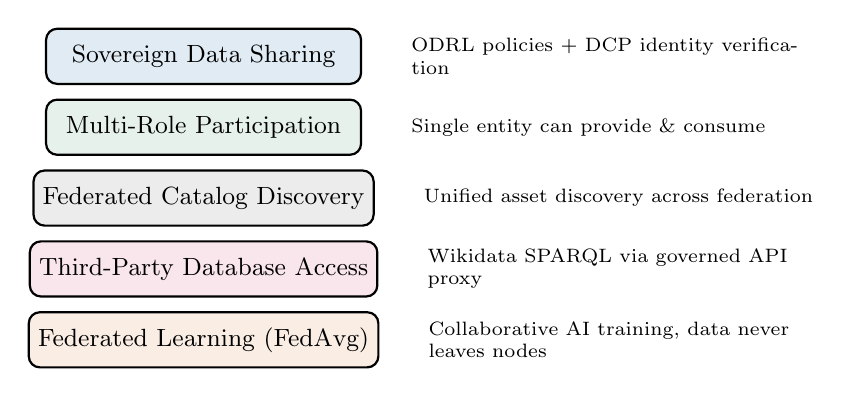
\begin{tikzpicture}[
  item/.style={draw, rounded corners, minimum width=4cm, minimum height=0.7cm, font=\small, thick, align=center},
]
  \node[item, fill=edcblue!12] (s1) at (0, 2.4) {Sovereign Data Sharing};
  \node[item, fill=edcgreen!12] (s2) at (0, 1.5) {Multi-Role Participation};
  \node[item, fill=gray!15]     (s3) at (0, 0.6) {Federated Catalog Discovery};
  \node[item, fill=purple!10]   (s4) at (0,-0.3) {Third-Party Database Access};
  \node[item, fill=edcorange!12](s5) at (0,-1.2) {Federated Learning (FedAvg)};

  \node[right=0.5cm of s1, font=\scriptsize, text width=5cm] {ODRL policies + DCP identity verification};
  \node[right=0.5cm of s2, font=\scriptsize, text width=5cm] {Single entity can provide \& consume};
  \node[right=0.5cm of s3, font=\scriptsize, text width=5cm] {Unified asset discovery across federation};
  \node[right=0.5cm of s4, font=\scriptsize, text width=5cm] {Wikidata SPARQL via governed API proxy};
  \node[right=0.5cm of s5, font=\scriptsize, text width=5cm] {Collaborative AI training, data never leaves nodes};
\end{tikzpicture}
\end{center}
\vspace{0.5em}
\begin{center}
\small Fully automated (Terraform + Python) \quad$\bullet$\quad Real-world data (OpenAlex, HN, Wikidata)
\end{center}

\vspace{1em}
\begin{center}
{\Large\bfseries Thank You}\\[0.5em]
{\large Questions?}
\end{center}
\end{frame}

\end{document}
